\chapter{Background and related work}
\label{cha:related}

Photovoltaic power forecasting relies on a broad range of time-series techniques, developed across operational statistics and modern machine learning. In practice, these methods face a shared challenge: separating the smooth diurnal cycle determined by solar geometry from sudden fluctuations driven by localized cloud cover. This chapter reviews the most established and widely used approaches for the task, organizing them by how they represent temporal dependencies and adapt to unfamiliar installations.

The survey spans four distinct modeling paradigms. It begins with operational statistical baselines, including persistence and clear-sky index forecasts, which define standard performance floors across utilities. It then covers machine learning models built on tabular feature representations, where gradient-boosted decision trees remain the prevailing operational benchmark. Next, it examines modern deep learning sequence architectures designed specifically for time series, comparing linear trend-residual decompositions, patched transformers, gated variable-selection networks, and cross-variable attention mechanisms. Finally, it reviews recent time-series foundation models adapted from large-scale pretraining, visual encoders, and multimodal systems that fuse numerical histories with sky observations. Each section outlines the structural assumptions of the corresponding method and its ability to transfer to unseen plants under disjoint evaluation.

\section{Numerical forecasting models}
\label{sec:rw-numerical}

The benchmark begins with methods that make different assumptions about temporal structure. Persistence, Smart Persistence, climatology, and seasonal naive forecasts establish how much of the target can be explained by the current state and the daily cycle. They matter because photovoltaic power has a strong astronomical envelope. A method that improves only on this envelope may appear accurate while missing the difficult cloud-driven changes. Among these references, Smart Persistence carries the observed clearness relationship forward while the deterministic solar envelope evolves~\cite{haurwitz}. It therefore separates the predictable envelope from the unpredictable sky and serves as the denominator of the skill score used throughout this thesis.

The benchmark also includes tabular and sequence predictors. Some learn from the training fleet; others bring an externally pretrained prior. Tabular models map the forecasting window into a flattened feature representation, testing whether non-sequential tree ensembles provide sufficient inductive bias. Supervised sequence models process temporal order directly, varying in patch tokenization, channel independence, and cross-variable attention mechanisms. Section~\ref{sec:baseline-implementations} details the configuration of each baseline.

\subsection{Smart Persistence: clearness-index baseline}
\label{sec:rw-smart-persistence}

Standard persistence assumes that future power equals the latest observed measurement, which fails as the sun rises or sets across the forecast horizon. Smart Persistence accounts for this predictable geometric progression by holding the ratio between observed power and clear-sky expectation constant. At forecast origin $t$, it calculates the clearness index $k_t = y_t / y_{\mathrm{cs},t}$, where $y_{\mathrm{cs},t}$ represents expected generation under clear-sky conditions from a deterministic solar model~\cite{haurwitz}. For future lead step $t+h$, the forecast scales the expected clear-sky generation by this recent ratio:

\[
\hat{y}_{t+h} = k_t \, y_{\mathrm{cs},t+h} = y_t \, \frac{y_{\mathrm{cs},t+h}}{y_{\mathrm{cs},t}}.
\]

This formulation separates atmospheric attenuation from astronomical motion. Because clear-sky irradiance is known in advance from solar geometry, Smart Persistence isolates how well a model anticipates actual cloud variation. In solar forecasting literature, it serves as the standard baseline for calculating skill scores~\cite{singh2026pvforecastreview}. Over short intervals up to an hour, local cloud conditions often persist and make this baseline competitive. Across multi-hour horizons, cloud fields move and evolve, so constant-clearness projections degrade. In this thesis, Smart Persistence provides the reference denominator for all skill score evaluations.

\subsection{LightGBM: gradient boosting over a feature table}
\label{sec:rw-lightgbm}

LightGBM~\cite{lightgbm} grows an ensemble of decision trees over lagged normalized power, calendar variables, and permitted meteorological covariates. Each split is an axis-aligned threshold, allowing the model to capture nonlinear cutoffs and interactions. In this benchmark, LightGBM provides a feature-table reference for testing how much predictive information the engineered inputs expose.

The transfer setting strains these assumptions. Temporal relationships are fixed before learning begins. LightGBM can discover that a particular lag matters, but it cannot construct intermediate states as an attention-based or recurrent model does. A learned threshold transfers only if its feature has a similar meaning at a held-out plant. LightGBM tests whether the engineered table is sufficient for accurate transfer.

\subsection{TabPFN: tabular foundation model}
\label{sec:rw-tabpfn}

TabPFN~\cite{tabpfn3} uses the same feature table without fitting a predictor on the target data. It applies a transformer pretrained across synthetic tabular tasks and predicts from a bounded in-context set of example rows. That setup is relevant when a new plant has little history and fitting a separate model is poorly posed.

TabPFN's bounded context means that a long, densely sampled corpus must be summarized into the rows and features the model accepts. The row-selection rule is therefore part of the method. Section~\ref{sec:baseline-implementations} specifies how it is applied across plants. The result tests how far a pretrained tabular prior can forecast from engineered numerical features without learning directly from the original sequence.

\subsection{DLinear and PatchTST: linear decomposition against patched attention}
\label{sec:rw-dlinear-patchtst}

DLinear~\cite{dlinear} decomposes each series into trend and seasonal components, projecting each with a single linear layer. It provides an efficient linear baseline that establishes how much predictive skill stems from capacity normalization and linear trend projection prior to applying transformer attention.

PatchTST~\cite{patchtst} segments univariate histories into temporal patches, reducing token count while capturing local sub-series dynamics. It processes channels independently, preventing spurious cross-variable correlations from overfitting to specific training sites. While channel independence aids cross-plant transfer, it precludes direct modeling of weather-power interactions. Patch tokenization also aggregates observations into multi-hour tokens, smoothing intra-patch fluctuations during steep ramp intervals.

\subsection{The Temporal Fusion Transformer: gating and variable selection}
\label{sec:rw-tft}

In contrast to PatchTST's channel-independent design, the Temporal Fusion Transformer~\cite{tft} combines recurrent processing, gated residual connections, explicit variable selection, and interpretable multi-horizon attention. It was designed for supervised settings in which known future inputs, observed past inputs, and static metadata coexist and vary in quality. This setup resembles a photovoltaic fleet, where some covariates are reliable at one site and noisy at another. The model's gates can in principle learn to suppress unhelpful covariates. It is included to test whether explicit input selection and a purpose-built multi-horizon decoder compensate for the absence of broad pretraining.

\subsection{iTransformer: variables as tokens}
\label{sec:rw-itransformer}

iTransformer~\cite{itransformer} inverts the usual transformer convention. Each physical variable becomes a token whose embedding spans the whole input window. Self-attention operates across variables rather than across time. In photovoltaic forecasting, generation, solar position, cloud cover, irradiance, temperature, and wind share substantial structure. The inversion lets the model relate these variables explicitly without inferring their relationship through a shared temporal representation. The token layout is shown in Figure~\ref{fig:related-itransformer}.

\begin{figure}[H]
\centering
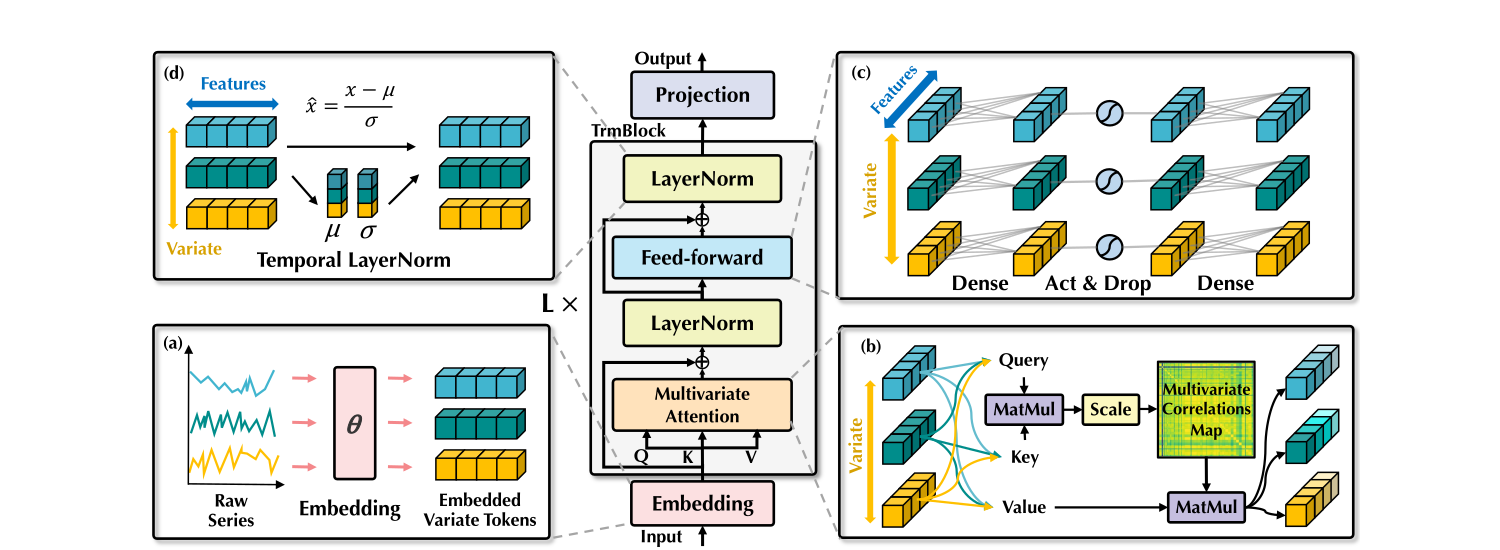
\includegraphics[width=0.94\textwidth]{figures/related_itransformer_original.png}
\caption{iTransformer architecture. Each variable is embedded as a token spanning the input window, and self-attention models relations across variables. Reproduced from the source architecture~\cite{itransformer}.}
\label{fig:related-itransformer}
\end{figure}

\section{Time-series foundation models}
\label{sec:rw-tsfm}

Time-series foundation models are pretrained on many series before zero-shot use or task adaptation. Chronos-2~\cite{chronos2}, TimesFM~\cite{timesfm}, TiRex~\cite{tirex}, and Tiny Time Mixer (TTM)~\cite{ttm} cover several architectural families. A model exposed to a broad corpus may bring useful temporal representations to a series it has never seen.

Their treatment of the input differs. Patch-based models compress a long context into blocks of observations. This makes long histories tractable, but can blur rapid behavior within a patch. Covariate support and output representations also differ across families, from point forecasts to quantile distributions.

Pretraining does not remove the need for a controlled comparison. Photovoltaic power has daily zeros, seasonality, cloud-driven ramps, and plant-to-plant variation that may not be represented in a general pretraining corpus. A zero-shot result measures the match between prior knowledge and this task. A fine-tuned result measures both that prior and the information obtained from the training fleet. This distinction is carried into every result table in Chapter~\ref{cha:results}, because the two quantities support different claims.

\subsection{Chronos-2: the shared numerical backbone}
\label{sec:rw-chronos2}

Chronos-2~\cite{chronos2} has a dual role in this thesis and therefore deserves a fuller description than the other checkpoints. It tokenizes a numerical history into fixed-length patches, processes them with a pretrained encoder, and emits quantiles for the forecast horizon in one pass. Figure~\ref{fig:chronos2-original-architecture} shows the original architecture. Patching keeps the sequence short enough for additional visual tokens, while the quantile head supports accuracy and calibration evaluation. The visual arms insert tokens into a backbone that was originally trained for numerical inputs.

\begin{figure}[H]
\centering
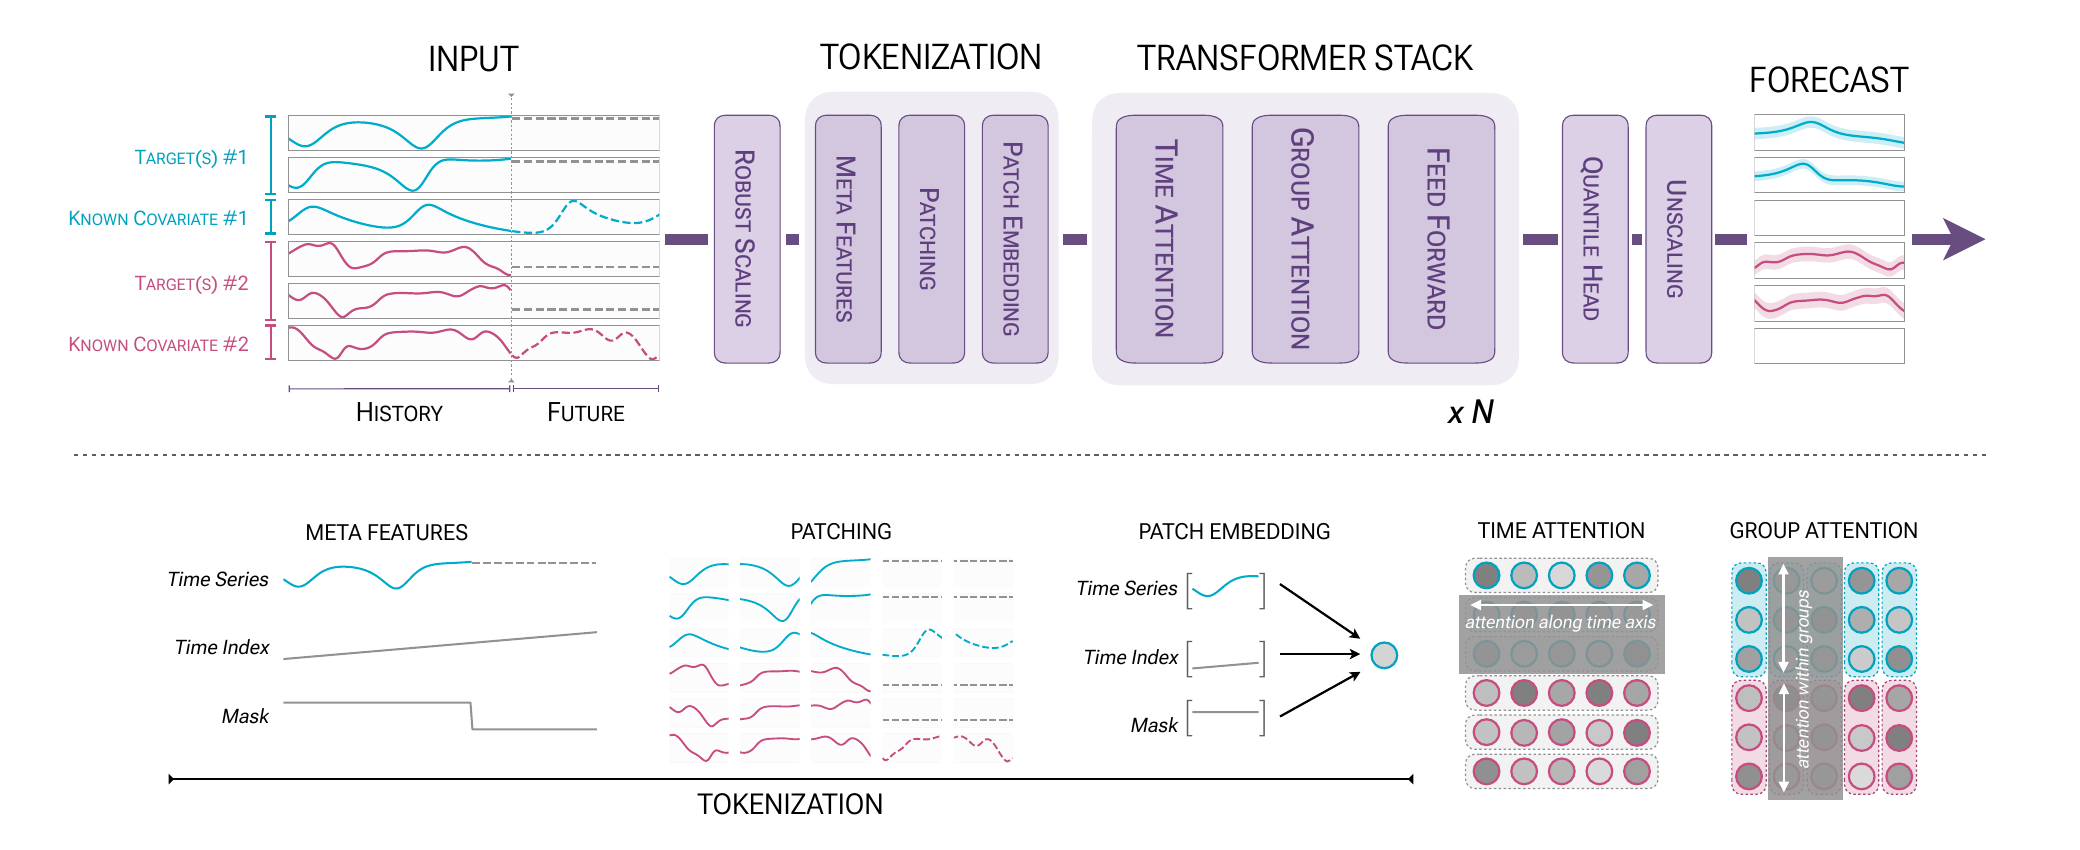
\includegraphics[width=\textwidth]{figures/chronos2_original_architecture.png}
\caption{Original Chronos-2 architecture, showing numerical input processing, the transformer backbone, and quantile forecasting. Reproduced from Figure 1 of the source paper~\cite{chronos2}.}
\label{fig:chronos2-original-architecture}
\end{figure}

The same checkpoint appears in the benchmark twice. Its zero-shot run tests how the released model performs on held-out plants before exposure to the training fleet. Fine-tuning it on the training plants produces the numerical baseline. The difference between these runs measures the benefit of in-domain adaptation from that pretrained starting point; it does not measure the value of pretraining itself. The numerical baseline is also the vision-free anchor of the fusion ladder. Each visual arm starts from its seed-matched adapted checkpoint.

\subsection{TimesFM, TiRex, and Tiny Time Mixer: breadth of temporal pretraining}
\label{sec:rw-tsfm-breadth}

The remaining foundation models provide task-level context across several architectures, showing how far off-the-shelf temporal pretraining reaches on this forecasting problem. TimesFM~\cite{timesfm} uses a decoder-oriented design intended for direct zero-shot forecasting at arbitrary horizons. TiRex~\cite{tirex} emphasizes in-context learning across varied horizon lengths. Tiny Time Mixer~\cite{ttm} replaces attention with lightweight mixing blocks. It targets a much smaller parameter budget, keeping both pretraining and adaptation cheap.

Together they show how released time-series checkpoints behave on plant-disjoint photovoltaic forecasting before fitting to the fleet. Photovoltaic power combines nightly zeros, a strong astronomical envelope, and ramps driven by an external process that the series records only after it reaches the plant. A weak zero-shot result therefore says more about the relation between the pretraining corpus and this task than about one architectural choice.

\section{Adaptation without a new model}
\label{sec:rw-adaptation}

Some methods adapt a pretrained time-series model without fully retraining it. Fine-tuning updates some or all backbone weights on the target fleet. Retrieval conditions a frozen forecaster on similar historical windows drawn from an external datastore. Alternatively, parameterized memory approaches such as MEMTS~\cite{memts} internalize domain-specific patterns directly into adapter parameters without requiring external database lookups during inference. Covariate adapters offer another route by injecting external inputs into an established representation through a small trainable path. These adaptation strategies offer lightweight alternatives to full end-to-end multimodal fine-tuning by modifying small parameter subsets or conditioning on retrieved instances.

\subsection{TS-RAG and Cross-RAG: retrieval as conditioning}
\label{sec:rw-retrieval}

TS-RAG~\cite{tsrag} and Cross-RAG~\cite{crossrag} retrieve related historical windows and make them available to a frozen or lightly adapted forecaster. Figure~\ref{fig:tsrag-original-architecture} shows the external-store interface in TS-RAG. Retrieval can supply examples of rare steep transitions at inference time without requiring the model weights to memorize them. The store can also grow without retraining the forecaster.

\begin{figure}[H]
\centering
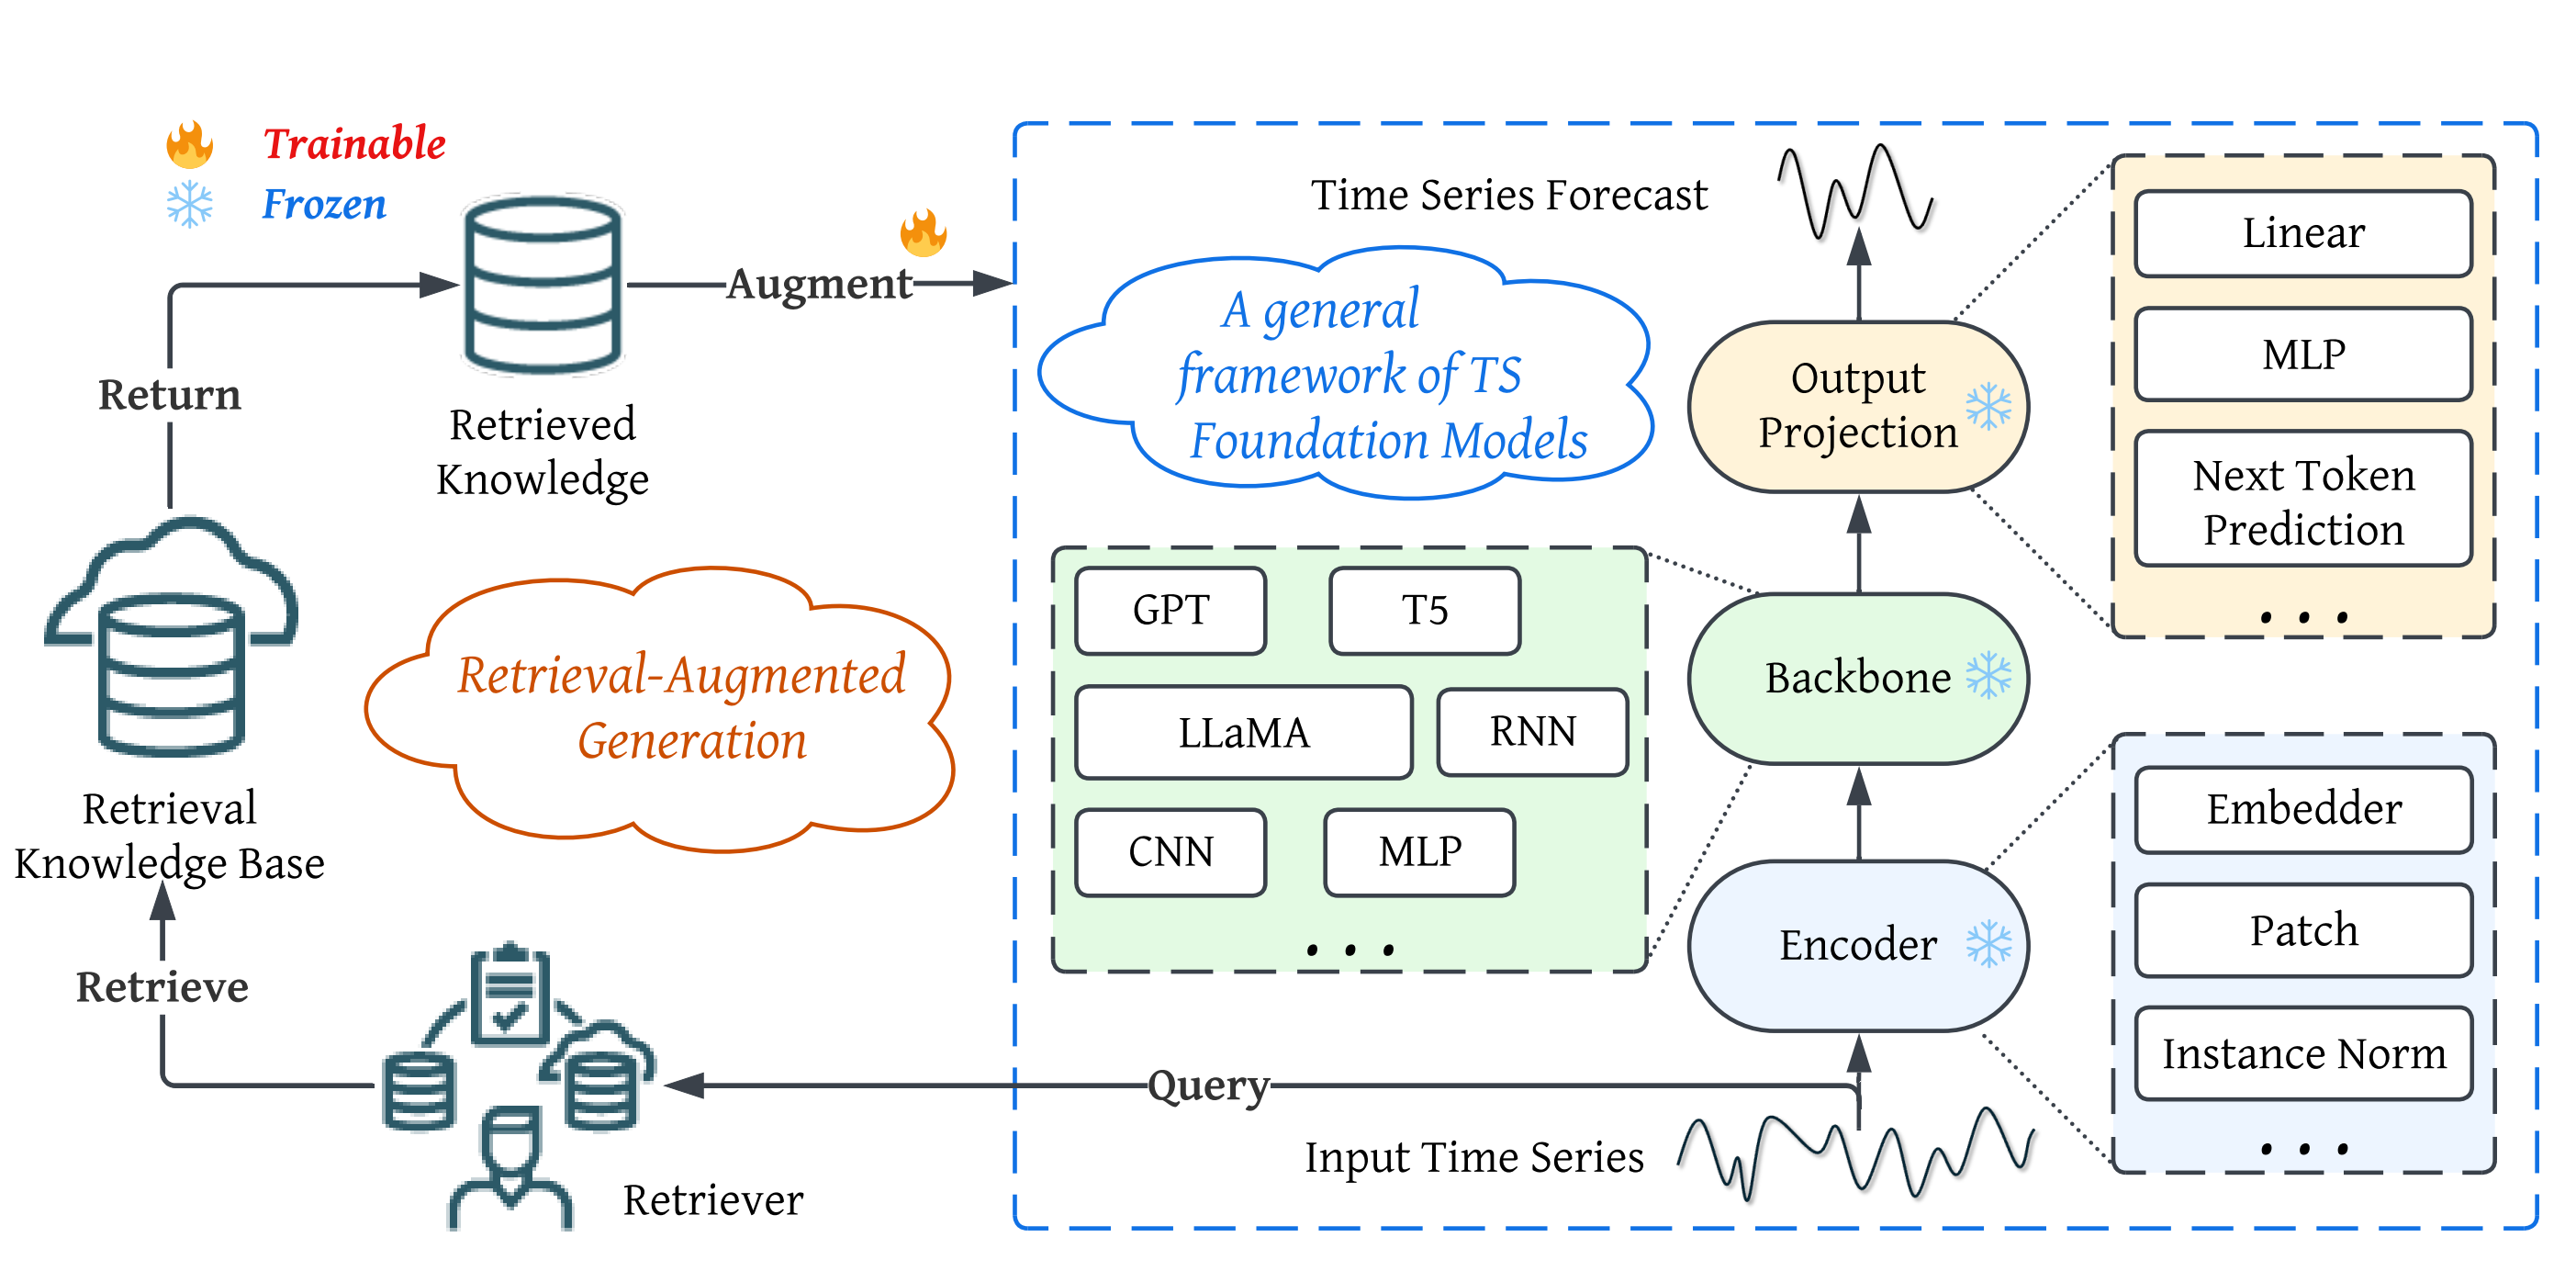
\includegraphics[width=\textwidth]{figures/tsrag_original_architecture.png}
\caption{TS-RAG overview from the source paper: a retriever supplies knowledge from an external store to a time-series foundation model while its backbone remains frozen~\cite{tsrag}.}
\label{fig:tsrag-original-architecture}
\end{figure}

Retrieval poses a specific risk for cross-plant evaluation. The method's effective training information is determined by the store's contents. A plant-disjoint protocol remains valid only if the store, the query construction, and the reported aggregate all respect the same entity boundary as the forecasting model.

\section{Multimodal forecasting interfaces}
\label{sec:rw-interfaces}

Multimodal forecasters use visual inputs in two ways. Time-series renderings let a vision encoder reinterpret measurements already present in the numerical history. Sky-camera and satellite images can add observations of the atmosphere that have not appeared in the power trace. The distinction matters when a forecast improves: a rendered image tests a new representation, while a real image may add new information whose use still needs to be measured.

\subsection{Time-VLM and VisionTS++: rendered time-series images}
\label{sec:rw-rendered}

Time-VLM~\cite{timevlm} and VisionTS++~\cite{visiontspp} render numerical history as an image and encode it with a visual backbone. Time-VLM also uses statistical text prompts; its paths appear in Figure~\ref{fig:related-time-vlm}. The rendered image may expose temporal patterns to a visual encoder, but it contains no observation beyond the numerical history used to construct it.

This distinction matters when interpreting a benchmark. A pseudo-image model can be a strong forecasting baseline because it tests a legitimate representation choice. It evaluates the value of re-encoding a history rather than the value of an independently observed modality.

\begin{figure}[H]
\centering
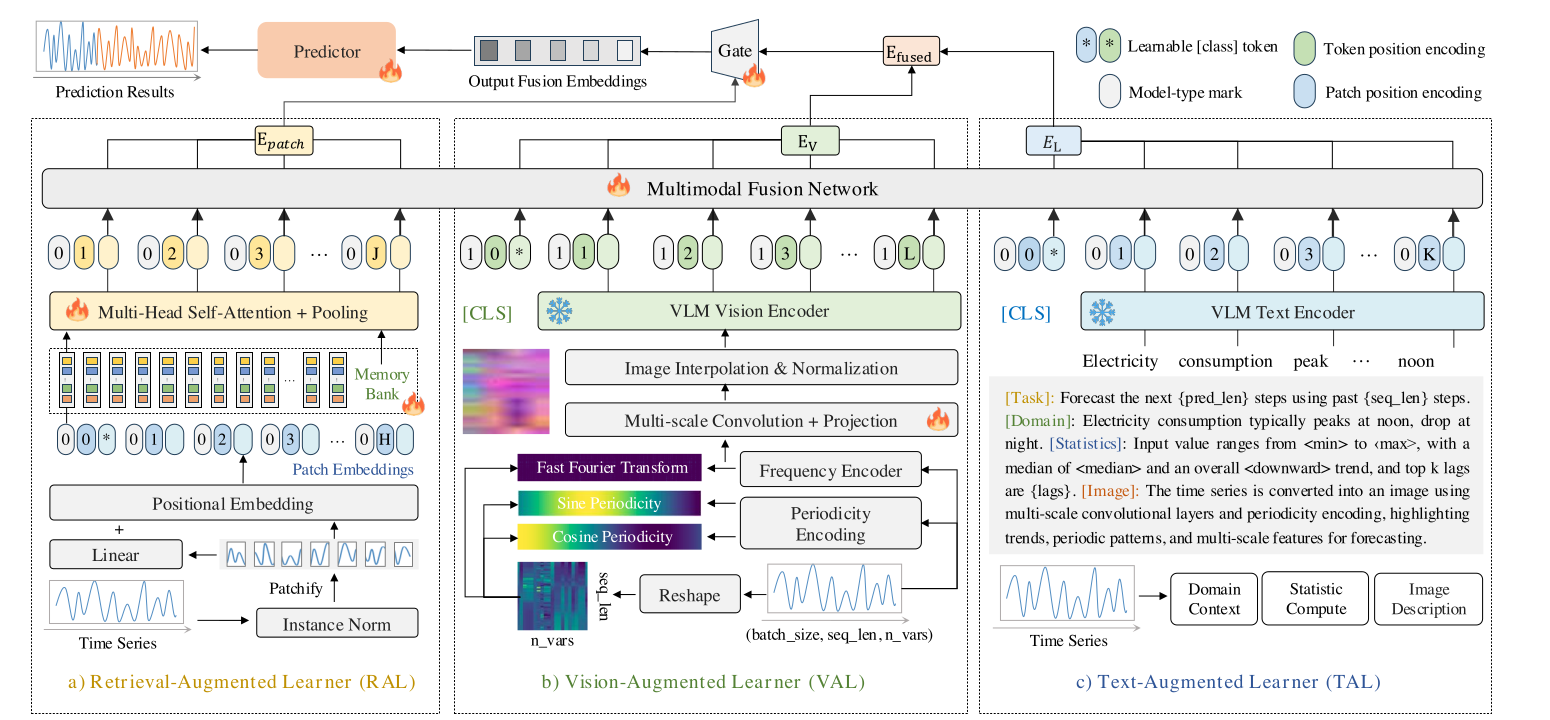
\includegraphics[width=0.94\textwidth]{figures/related_time_vlm_original.png}
\caption{Time-VLM architecture. Historical time-series values are rendered as an image and combined with statistical text prompts before forecasting. Reproduced from the source architecture~\cite{timevlm}.}
\label{fig:related-time-vlm}
\end{figure}

\subsection{Aurora: pretraining across derived modalities}
\label{sec:rw-aurora}

Aurora~\cite{aurora} extends this line of work to multimodal foundation-model pretraining. It combines modality-specific encoders with a cross-modality encoder that uses token distillation and modality-guided self-attention, as shown in Figure~\ref{fig:related-aurora}. Its training uses numerical series, images derived from those series, and text descriptions. The resulting model tests whether these representations improve general forecasting behavior and transfer.

\begin{figure}[H]
\centering
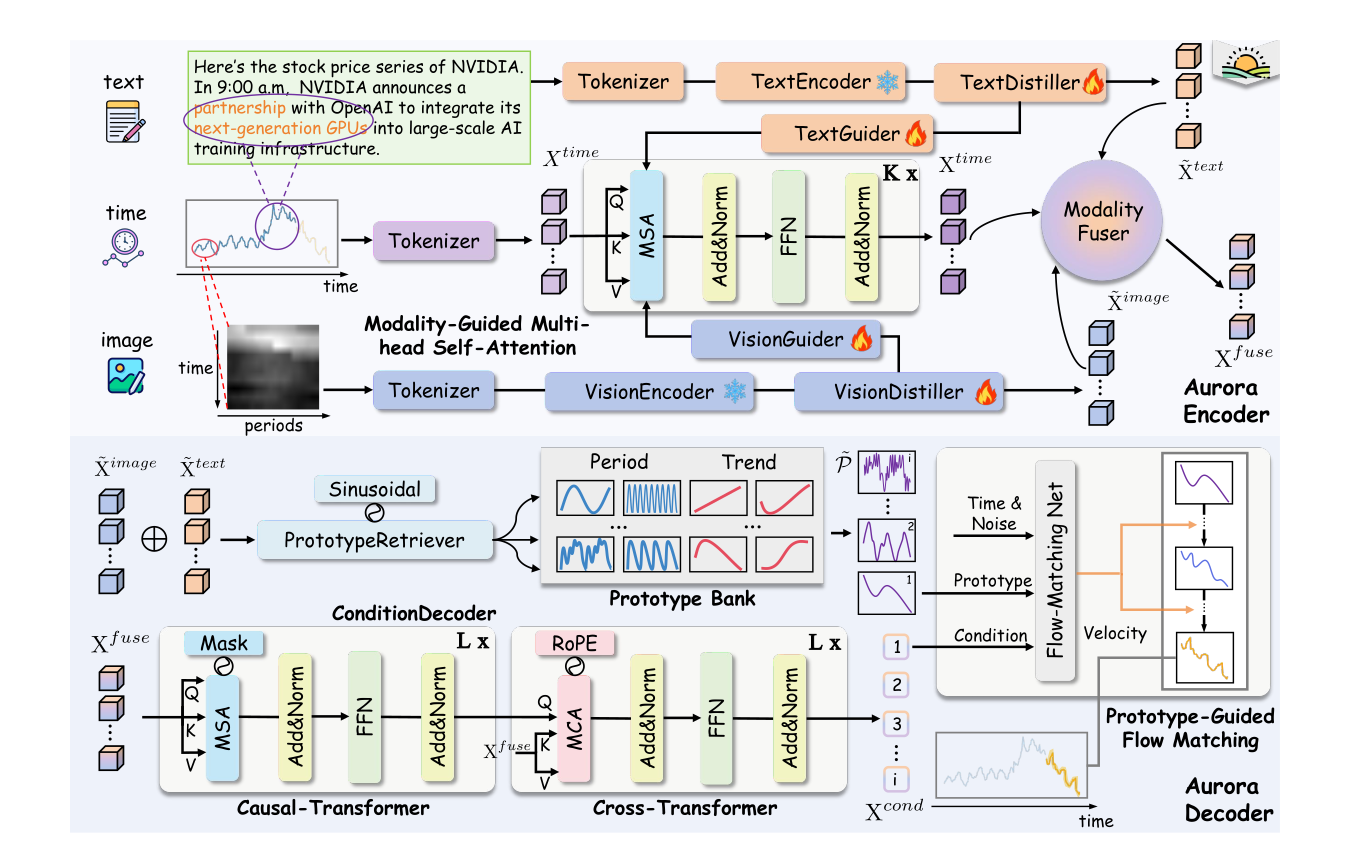
\includegraphics[width=0.94\textwidth]{figures/related_aurora_original.png}
\caption{Aurora architecture. Modality-specific encoders feed a cross-modality encoder that uses token distillation and modality-guided self-attention. Reproduced from the source architecture~\cite{aurora}.}
\label{fig:related-aurora}
\end{figure}

\subsection{SUNSET: a photovoltaic convolutional reference}
\label{sec:rw-sunset}

SUNSET was an early end-to-end model for forecasting photovoltaic power from ground-based sky-image sequences and recent power output~\cite{sunsetearly}. The forecasting architecture stacks successive frames along the image channel dimension and extracts visual features with two convolutional blocks. It inserts the power history after image processing and uses fully connected layers to predict 15-minute-ahead output~\cite{sunset}. Its released implementation has made it a recurring reference in image-based forecasting comparisons, including the SKIPP'D benchmark~\cite{skippd}, providing an established convolutional baseline for comparison with modern foundation-model interfaces. Subsequent studies expanded ground-based sky observation using generative video modeling in SkyGPT~\cite{skygpt} and multimodal vision-language architectures in PV-VLM~\cite{pvvlm}, while multi-scale fusion networks such as M3S-Net~\cite{m3snet} combine local telemetry with multi-scale image features.

\subsection{Solar-VLM: gated late fusion}
\label{sec:rw-solarvlm}

Solar-VLM~\cite{solarvlm} combines a visual pathway for satellite crops with meteorological text and a time-series pathway. As shown in Figure~\ref{fig:related-solar-vlm}, transformer blocks and weighted temporal aggregation summarize the visual sequence. A KNN/GAT pathway models relations among sites, and cross-site attention integrates that spatial context. The resulting visual and meteorological representation is fused with the time-series state through a learned gate. The architecture therefore includes temporal and cross-site processing in addition to station-level fusion. For the present comparison, the relevant distinction is that the forecaster receives an aggregated representation rather than a sequence of individually addressable satellite patches.

Figure~\ref{fig:related-solar-vlm} shows the pooled station representation and gate in Solar-VLM.

\begin{figure}[H]
\centering
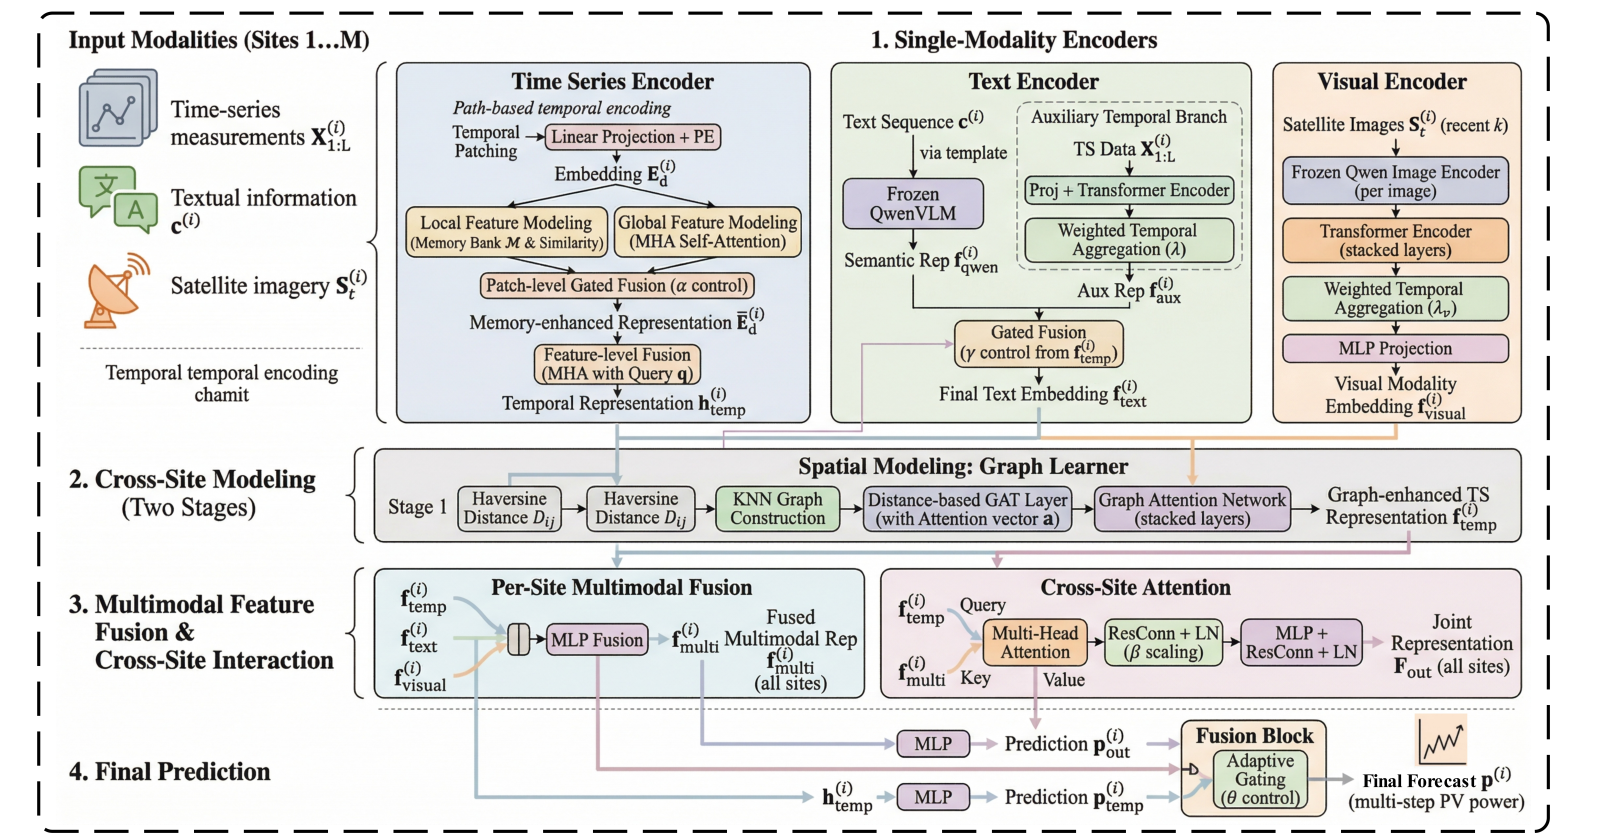
\includegraphics[width=0.94\textwidth]{figures/related_solar_vlm_original.png}
\caption{Solar-VLM architecture. The diagram shows visual temporal aggregation, KNN/GAT cross-site processing, cross-site attention, and gated fusion with the time-series branch. Reproduced from the source architecture~\cite{solarvlm}.}
\label{fig:related-solar-vlm}
\end{figure}

\subsection{PV-LLM: satellite and text prompts inside a language backbone}
\label{sec:rw-pvllm}

PV-LLM~\cite{pvllm} carries the prompting idea into a pretrained language model, replacing the time-series backbone. It uses a frozen GPT-2 and three input channels. A temporal-semantic encoder maps power and numerical weather history into embeddings aligned with the word space. A text prompt contains plant coordinates, forecast start time, dataset and task descriptions, and input statistics. A satellite encoder uses a context compressor to reduce the patch grid of each frame to a single vector. Figure~\ref{fig:related-pv-llm} shows these separate paths. Satellite features enter every self-attention layer through adaptive prompt-tuning blocks, whose gates start at zero. In its reported benchmark, the system is trained and evaluated on MMSP(S), a ten-plant Shandong subset of the same MMSP corpus released with FusionSF, with Himawari imagery and ECMWF forecasts at hourly resolution. It reports lower error than unimodal transformers, MLP mixers, Time-LLM, and FusionSF.

The context compressor leaves one vector per frame, so image locations are no longer available as separate tokens inside GPT-2. The vector may still encode spatial information. The paper's prompt ablation finds larger gains from forecast start time and plant coordinates than from its other text components. Those gains concern metadata conditioning and do not establish which satellite content the model uses. Although coordinates can be available for a held-out plant, PV-LLM's reported evaluation does not test plant-disjoint transfer; its results are for easy and hard test windows. The cross-track result in this thesis evaluates different MMTSFM arms on eight held-out US plants. It does not change the scope of PV-LLM's published evidence.

\begin{figure}[H]
\centering
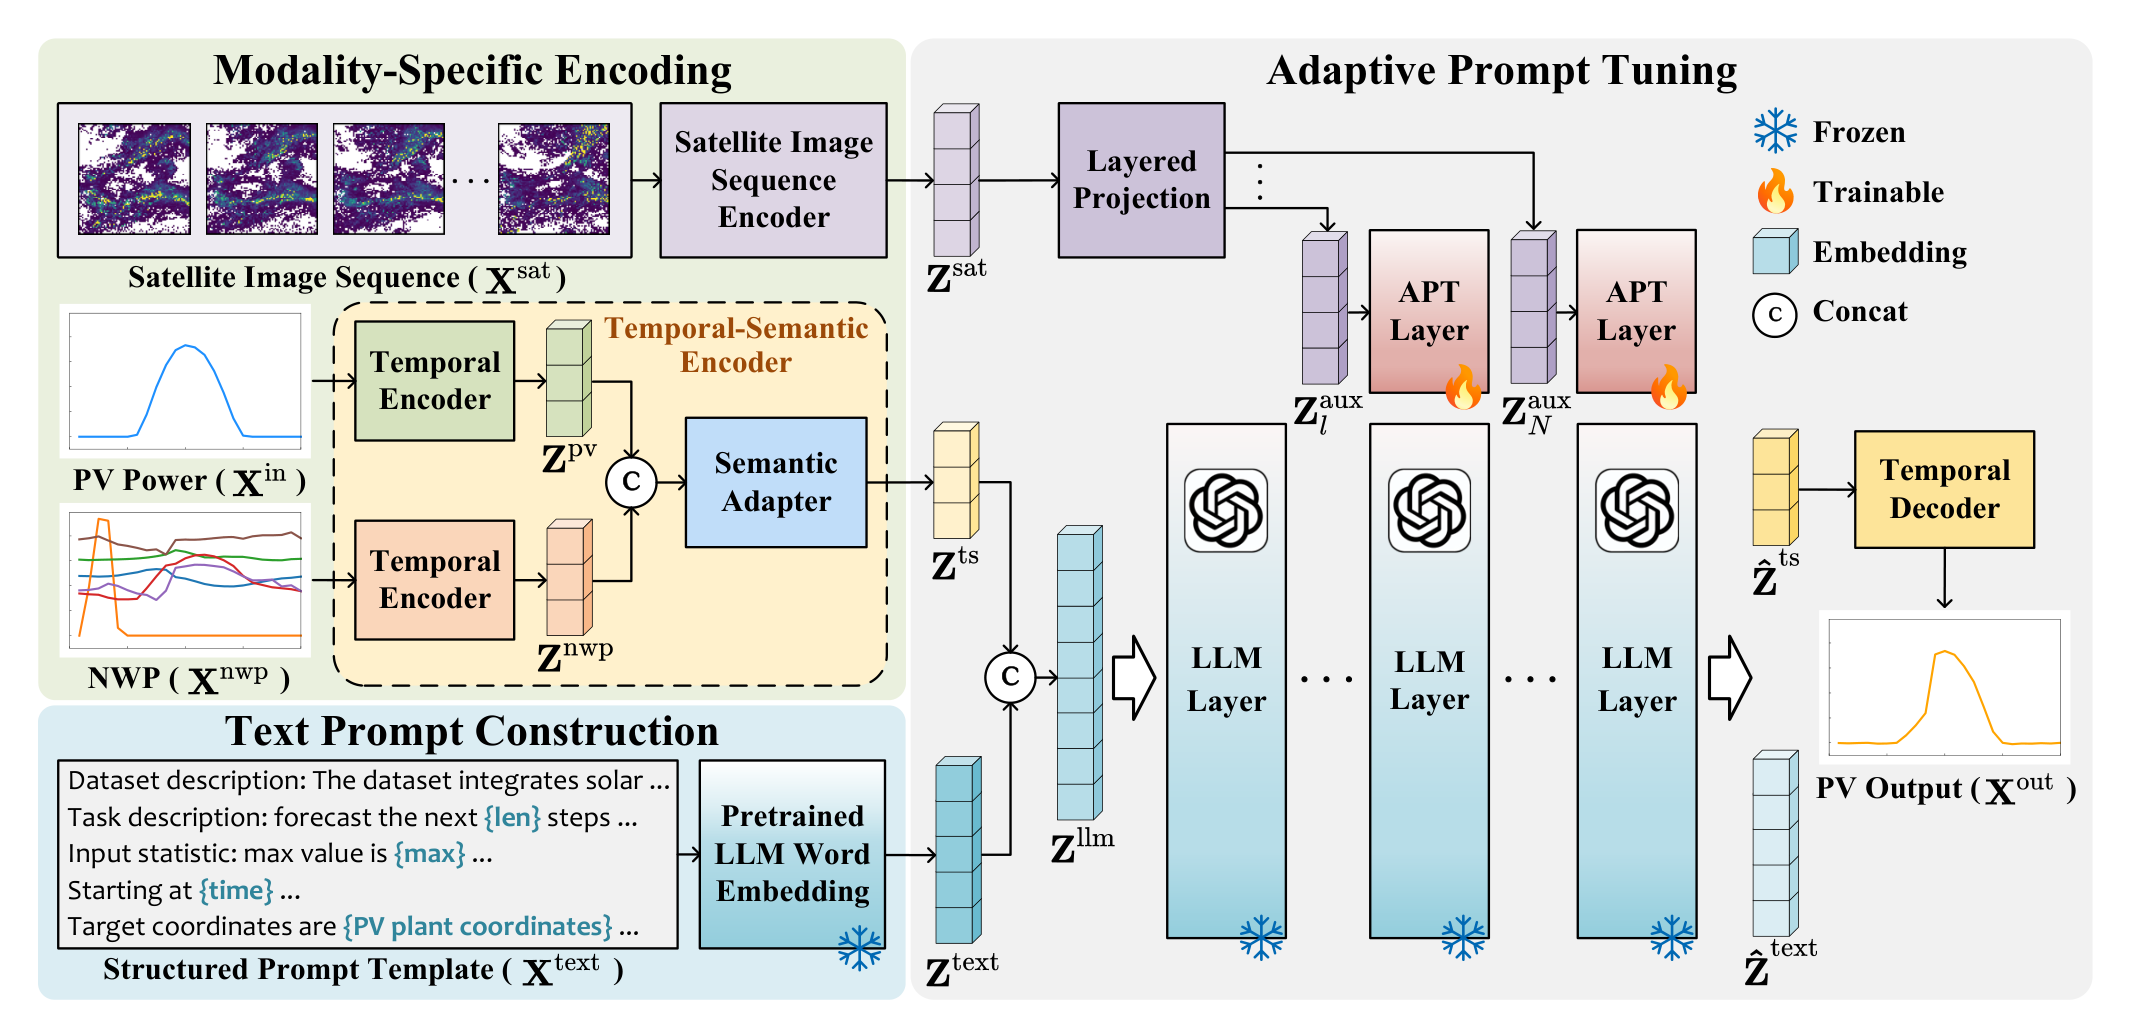
\includegraphics[width=0.96\textwidth]{figures/related_pv_llm_original.png}
\caption{PV-LLM architecture. Satellite frames, power and numerical weather history, and a structured text prompt are encoded separately. The text and time-series embeddings enter a frozen language model directly, while satellite embeddings are injected at each layer through adaptive prompt-tuning blocks. Reproduced from the source architecture~\cite{pvllm}.}
\label{fig:related-pv-llm}
\end{figure}

\section{Nemotron 3 Nano Omni: visual token selection}
\label{sec:rw-nemotron}

Nemotron 3 Nano Omni~\cite{nemotron} is a multimodal model outside photovoltaic forecasting. Its visual pathway reduces features by spatial downsampling and then selects tokens from regions that change over time, as shown in Figure~\ref{fig:related-nemotron}. Efficient Video Sampling~\cite{evs} supplies the selection step by pruning temporally redundant video tokens. This thesis draws on the resulting interface principle: reduce the visual token count while keeping selected locations distinct for the downstream backbone.

\begin{figure}[H]
\centering
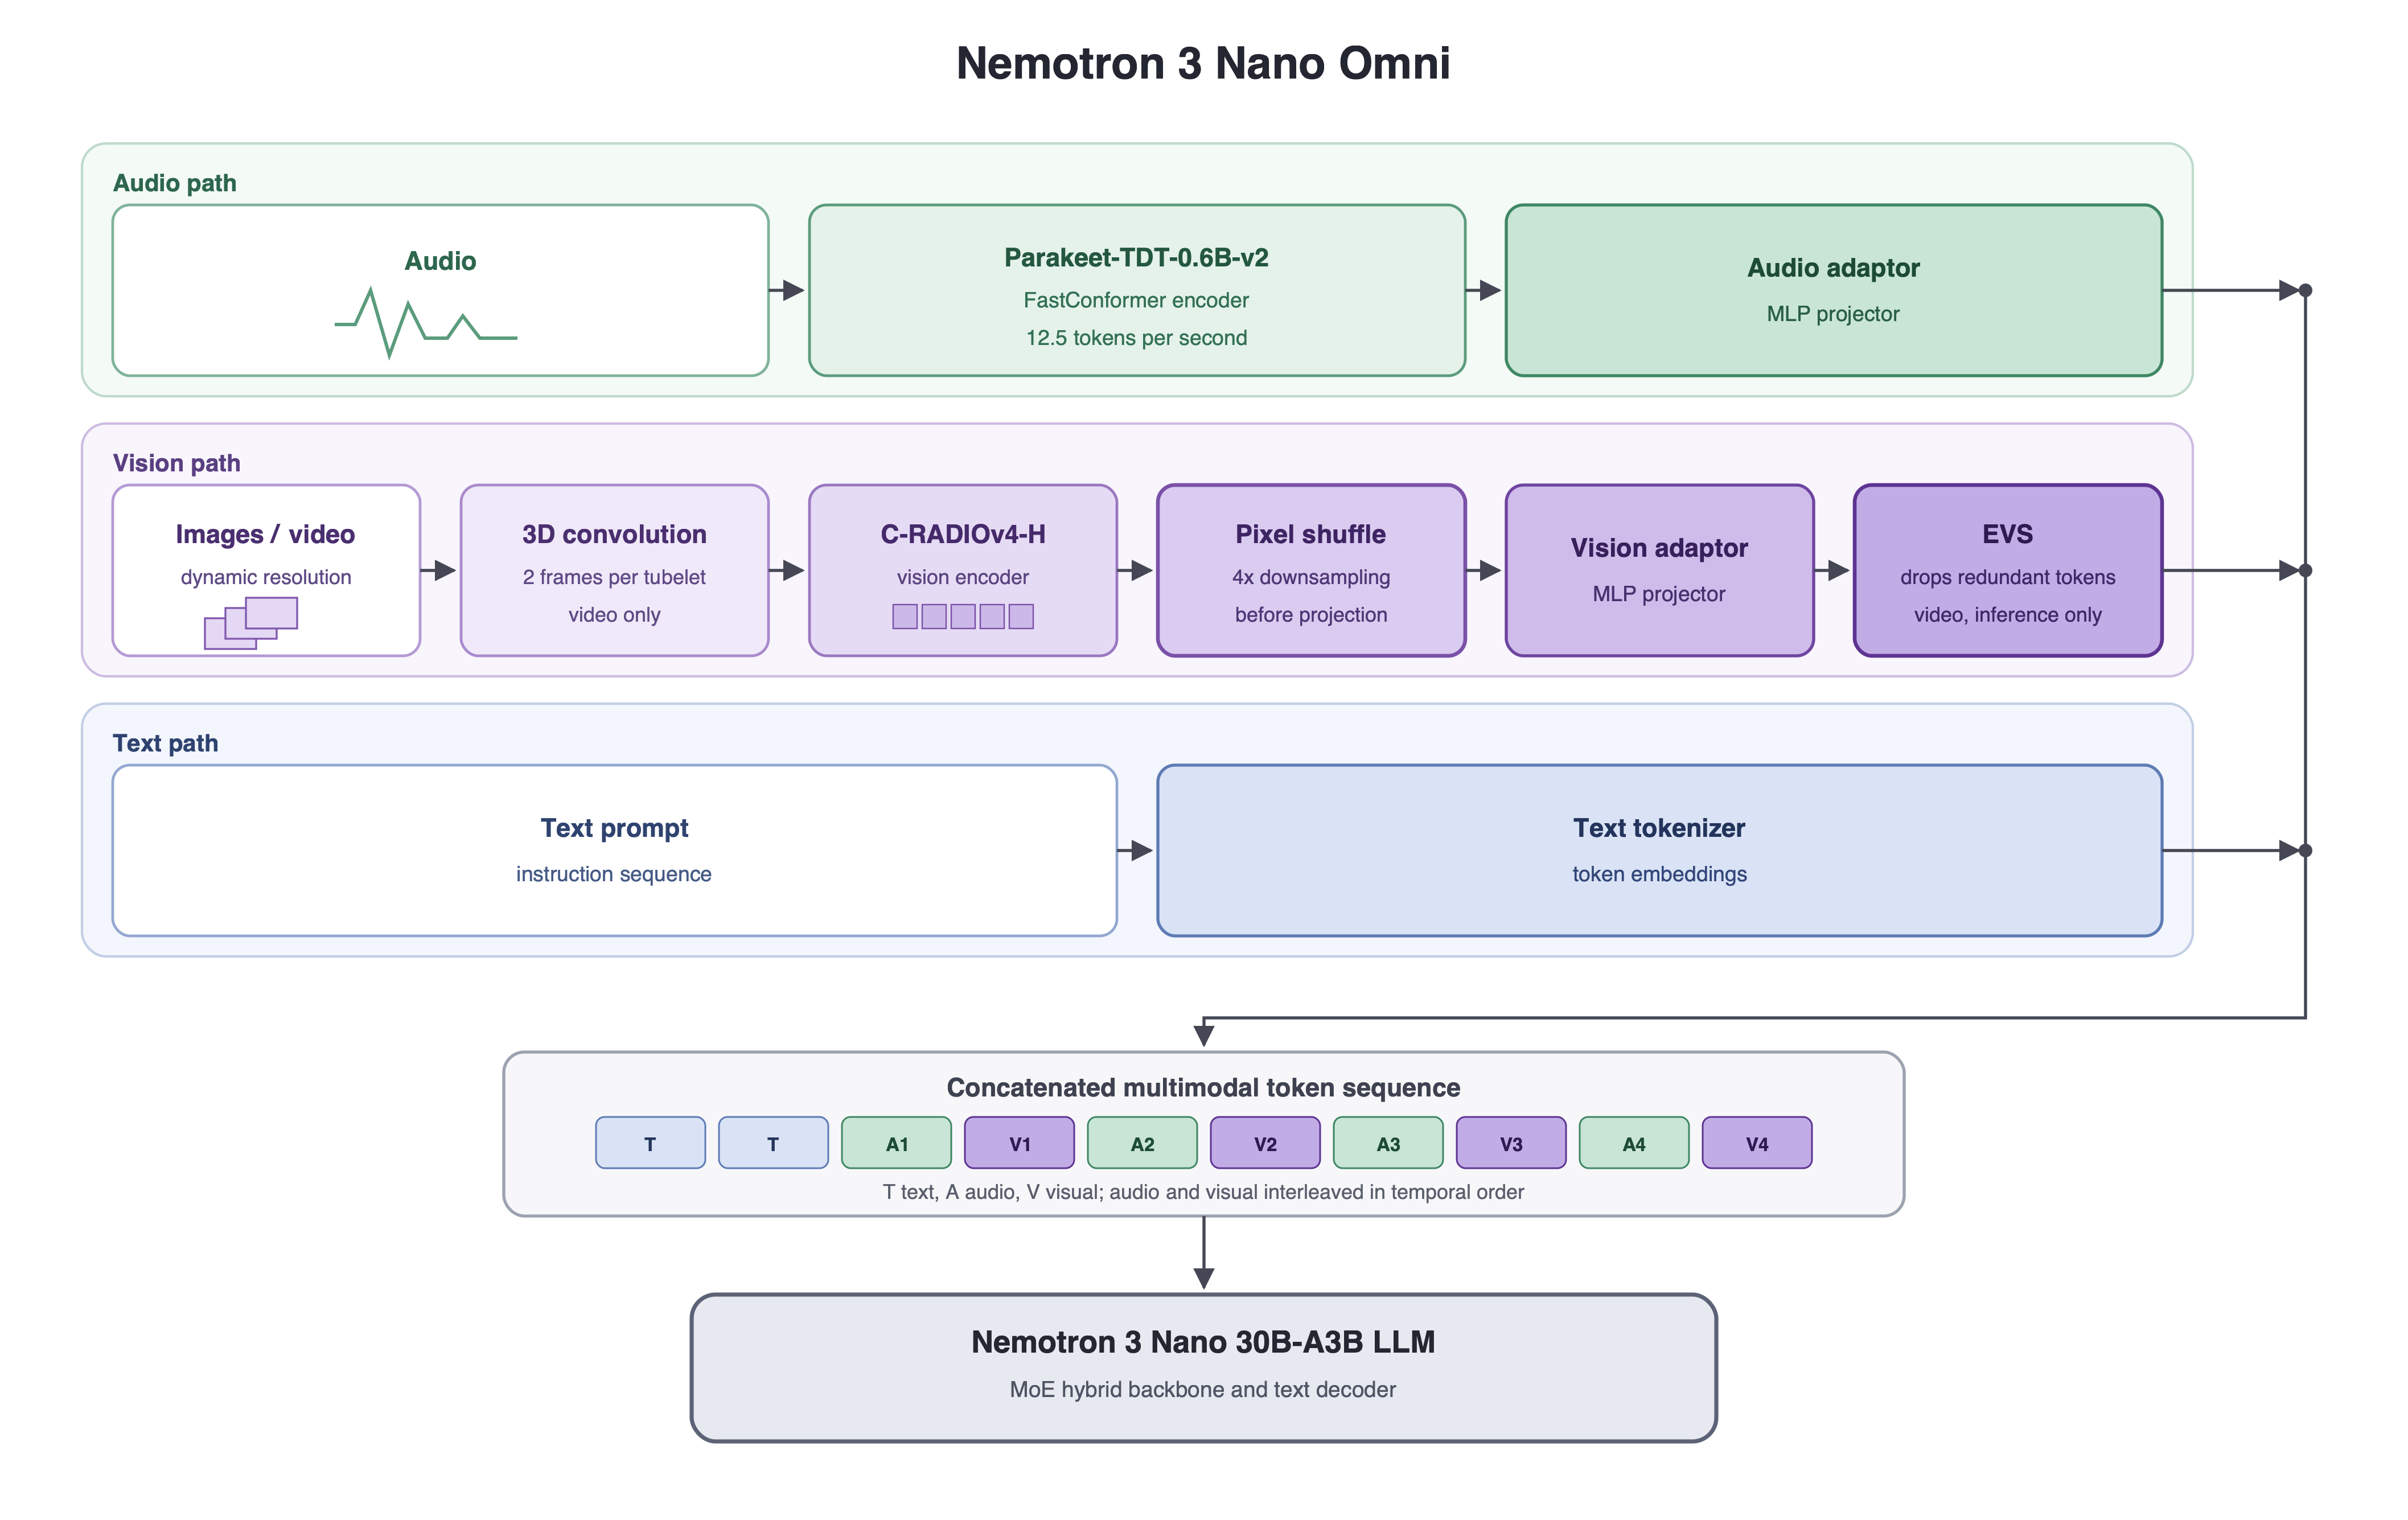
\includegraphics[width=0.92\textwidth]{figures/related_nemotron_visual_path.png}
\caption{Nemotron 3 Nano Omni visual pathway. The visual encoder produces tokens that are spatially reduced and then sampled before projection into the shared backbone. Reproduced from the source architecture~\cite{nemotron}.}
\label{fig:related-nemotron}
\end{figure}

\section{V-JEPA 2.1: dense video representations}
\label{sec:rw-vjepa21}

V-JEPA 2.1~\cite{vjepa21}, built on the self-supervised joint-embedding predictive architecture introduced in V-JEPA 2~\cite{vjepa2}, is trained on large collections of images and video. Its dense predictive objective trains on both visible and masked tokens, with additional supervision at intermediate encoder layers. The resulting representations retain spatial structure and temporal information while supporting global scene understanding. Unlike a single embedding for each frame, its patch features leave individual image regions available to a downstream model.

Figure~\ref{fig:related-vjepa21} shows the training architecture. Separate image and video tokenizers feed a shared context encoder; a predictor learns from both masked and visible tokens against targets from a teacher encoder.

\begin{figure}[H]
\centering
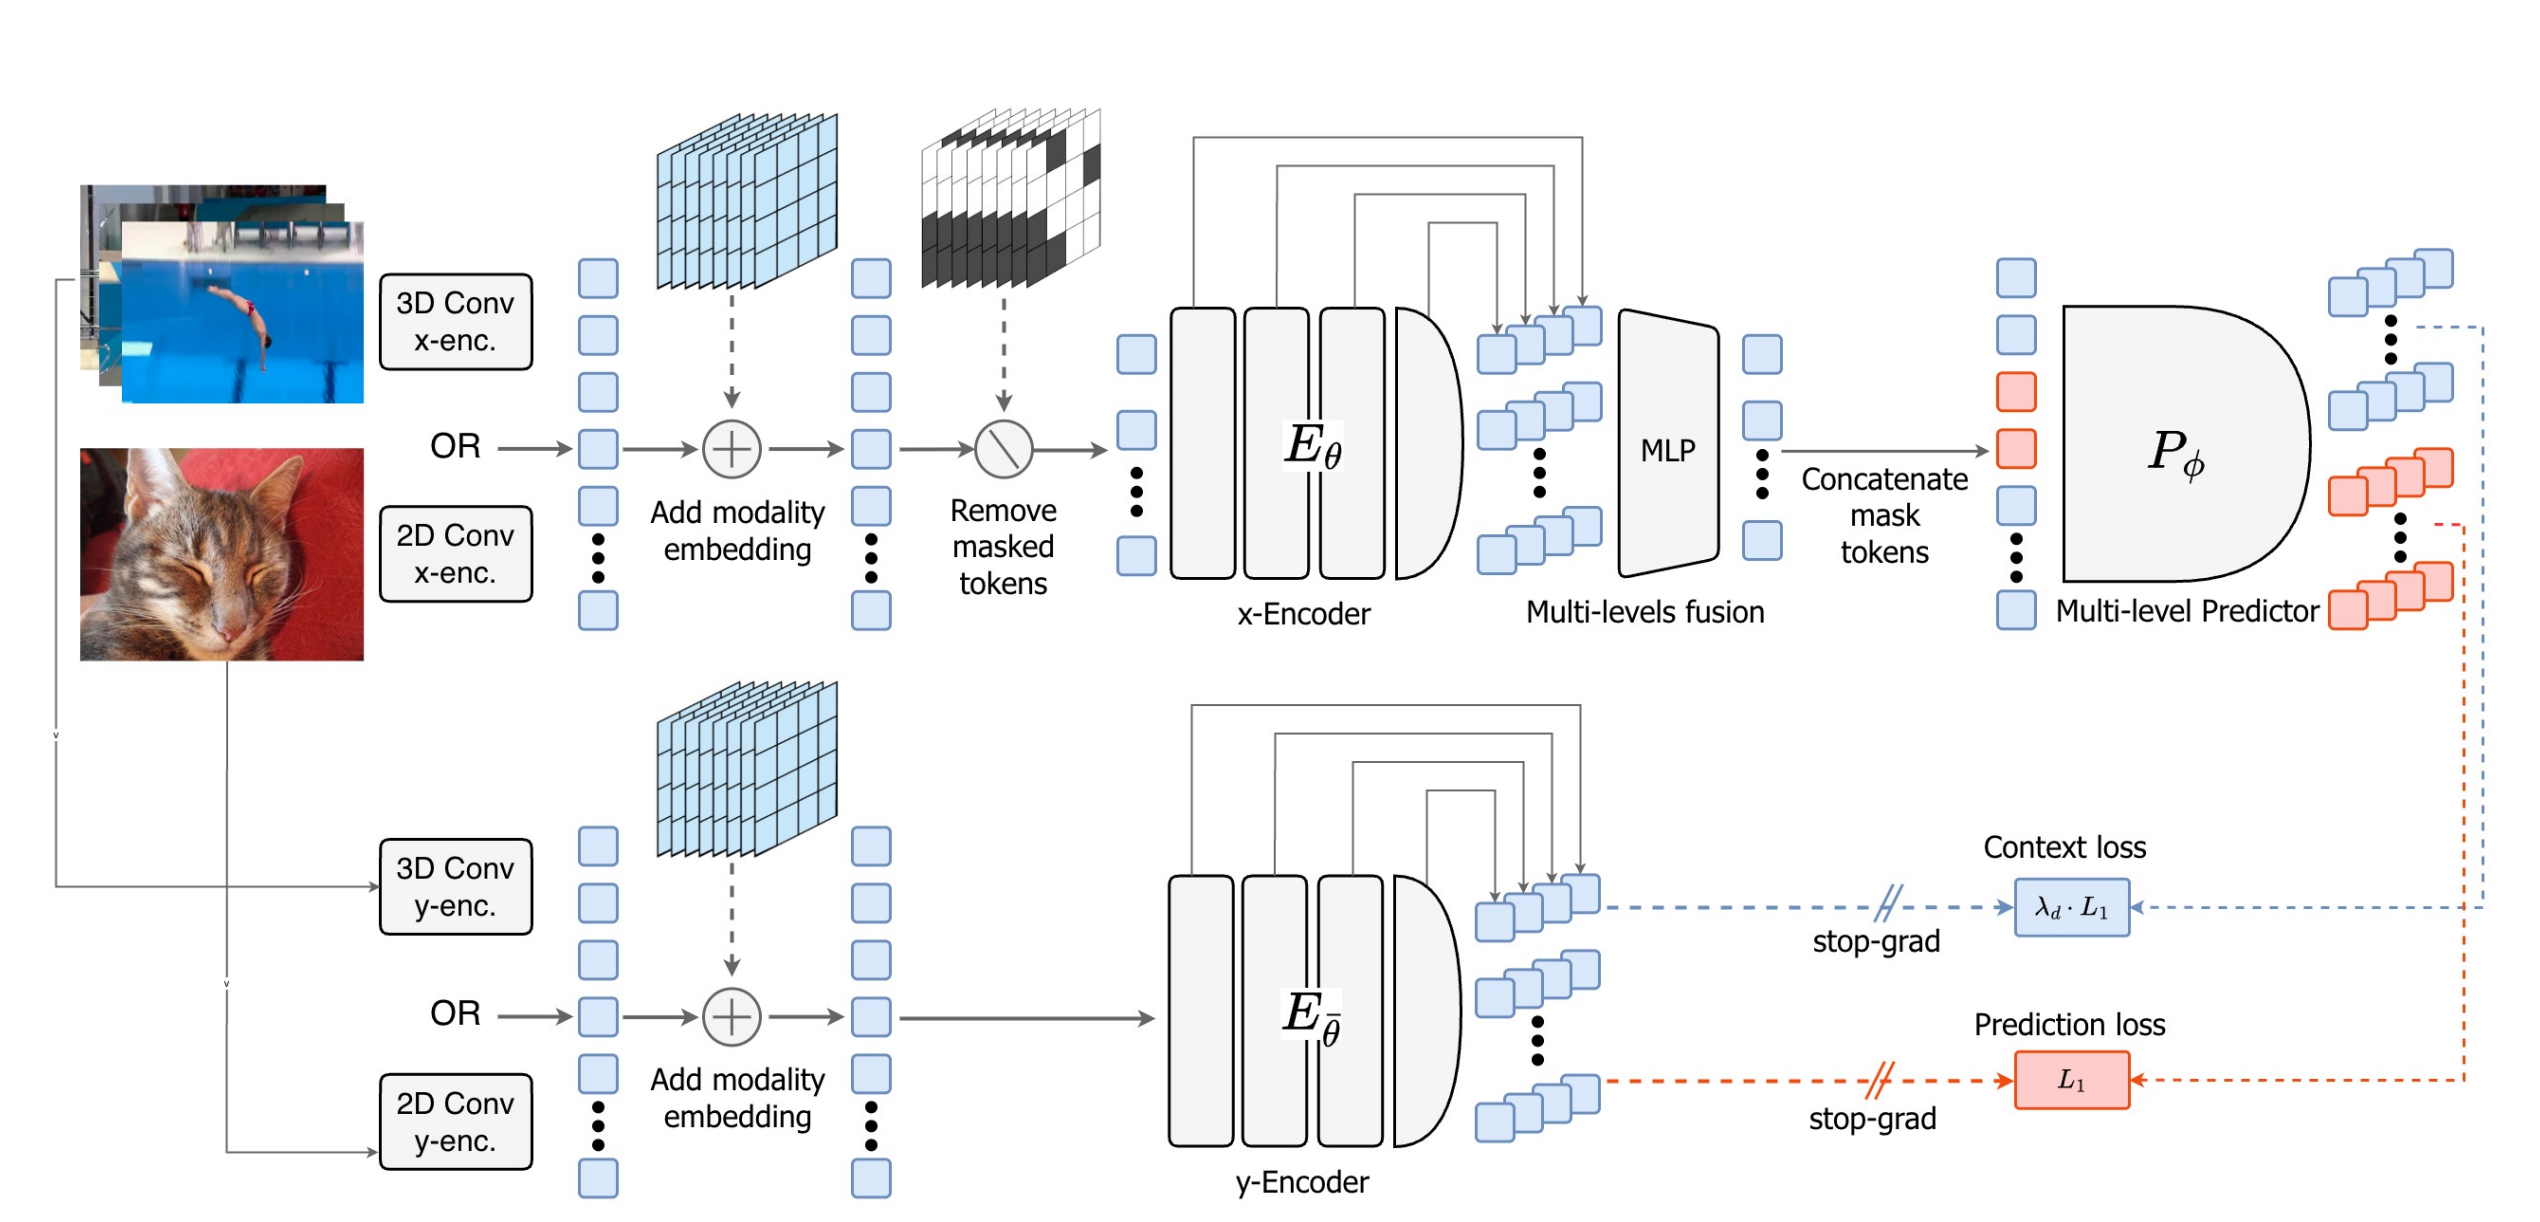
\includegraphics[width=0.96\textwidth]{figures/related_vjepa21_architecture.png}
\caption{V-JEPA 2.1 training architecture. Image and video inputs use separate tokenizers before the context and target encoders. Multi-level predictions are supervised at masked and visible token positions. Reproduced from the source architecture~\cite{vjepa21}.}
\label{fig:related-vjepa21}
\end{figure}

This thesis pairs a frozen V-JEPA 2.1 encoder with Chronos-2. Nemotron motivates the selection interface, while V-JEPA 2.1 supplies the visual features.
